{\color{Blue}{\subsection{AXI Protocol}}}

The AMBA AXI protocol supports high-performance, high-frequency system designs for communication between
multi masters and multi slaves components.
{\bf AXI4} is widely adopted, providing {\bf benefits} to {\bf productivity} (standardization simplifies the work of developers), {\bf flexibility} (there are slightly different protocols, eachone of them with their peculiarity), and {\bf availability} (it's an industrial standard, and there is a world wide community that uses and support it).
\newline

{\bf AXI4-Lite}, the procol that we studied, is a {\bf subset of AXI4} for communication with simpler control register style interfaces within components.
\newline

Some {\bf key features} of the AXI4-Lite protocol are: {\bf separate address/control and data phases}, support for unaligned data transfers, using byte strobes, {\bf separate read and write data channels}, all {\bf transactions} are of burst {\bf length 1}, all data accesses are non-modifiable, non-bufferable and use the full {\bf width of the data bus} (the supported busses are the ones with width of {\bf 32-bit} (in our case) or 64-bit), exclusive accesses are not supported.
\newline

One of the features of {\bf AXI4-Lite} is the {\bf Handshake protocol}, that is done {\bf for each payload exchanged and address line} and it ensures the reading of the right values. The signals involved are {\bf valid}, asserted by the sender, when the data is stable and available, and {\bf ready}, asserted by the reciever, when it is able to recieve the information. For more detailed explaination, please see \cite[Section-A3.2.1]{AXISpecification}.

\begin{figure}[!ht]
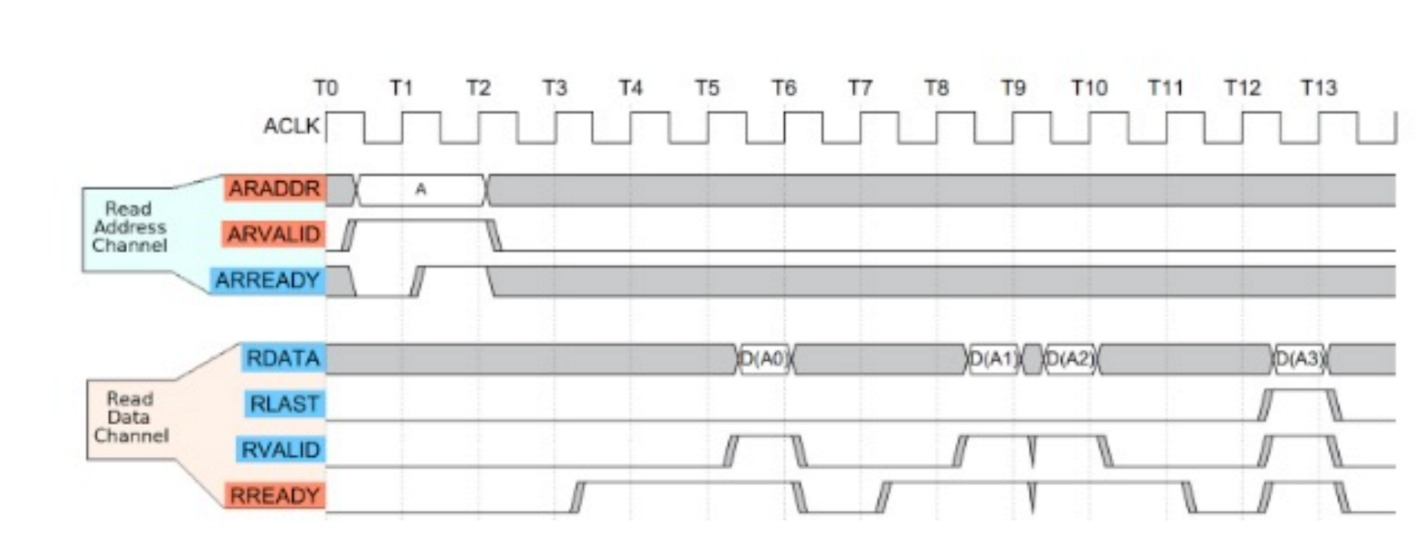
\includegraphics[width=1\textwidth]{./../../img/Images/axi_simple_read}
\caption{AXI4 ({\bf non lite}) read}
\label{simple_read}
\end{figure}
\begin{figure}[!ht]
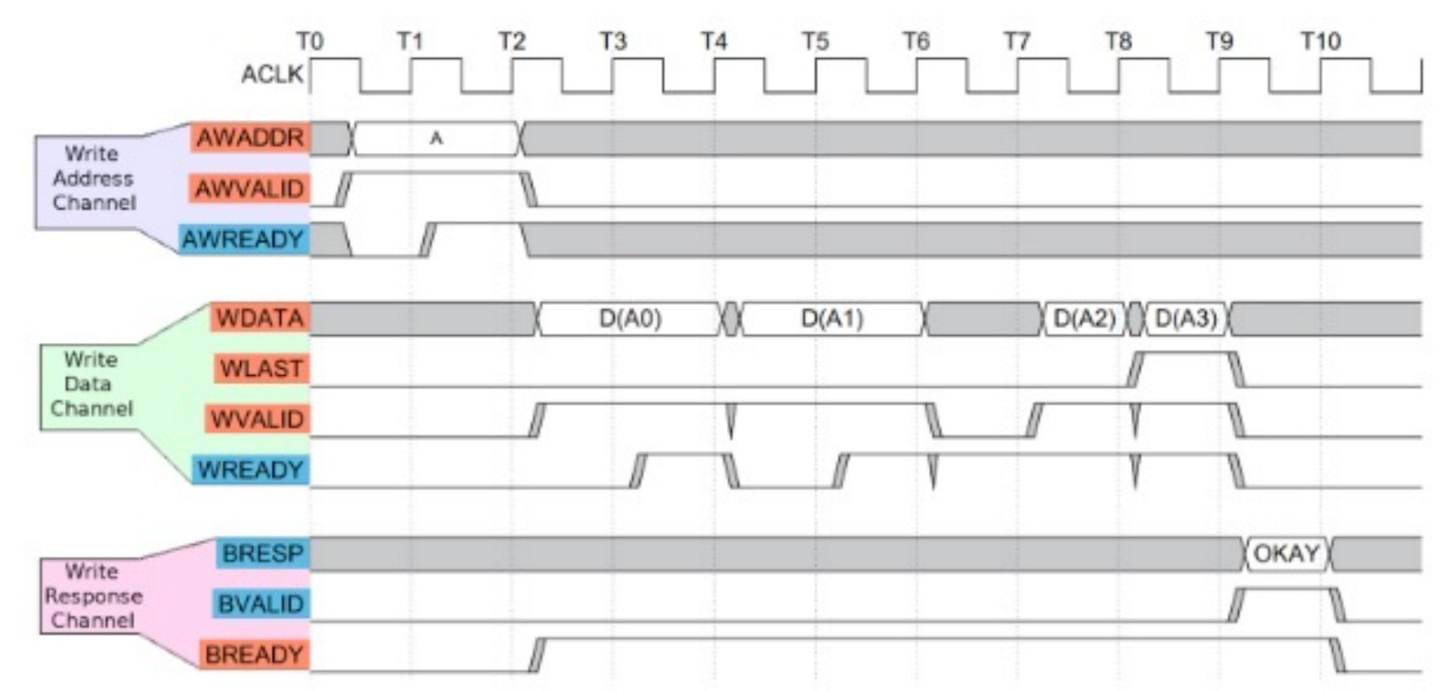
\includegraphics[width=1\textwidth]{./../../img/Images/axi_simple_write}
\caption{AXI4 ({\bf non lite}) write}
\label{simple_write}
\end{figure}

\begin{tabular} {c c l}
  \hline
  \multicolumn{3}{c}{\Large{WRITE SIGNALS}} \\

  \multicolumn{3}{c}{{AW group}} \\
  \textcolor{Red}{\small{AWADDR}} & \textcolor{Red}{\small{[31:0]}} & \textcolor{Red}{\small{//where the master want to write}} \\
  \textcolor{Red}{\small{AWVALID}} & \textcolor{Red}{\small{[0:0]}} & \textcolor{Red}{\small{//the address line is valid}} \\
  \textcolor{Red}{\small{AWPROT}} & \textcolor{Red}{\small{[2:0]}} & \textcolor{Red}{\small{//access permissions}} \\
  \textcolor{Blue}{\small{AWREADY}} & \textcolor{Blue}{\small{[0:0]}} & \textcolor{Blue}{\small{//the slave is ready to recieve the address}} \\

  \multicolumn{3}{c}{{W group}} \\
  \textcolor{Red}{\small{WDATA}} & \textcolor{Red}{\small{[31:0]}} & \textcolor{Red}{\small{//what the master want to write}} \\
  \textcolor{Red}{\small{WSTRB}} & \textcolor{Red}{\small{[3:0]}} & \textcolor{Red}{\small{//which bytes of the WDATA are meaningful}} \\
  \textcolor{Red}{\small{WVALID}} & \textcolor{Red}{\small{[0:0]}} & \textcolor{Red}{\small{//the data line is valid}} \\
  \textcolor{Blue}{\small{WREADY}} & \textcolor{Blue}{\small{[0:0]}} & \textcolor{Blue}{\small{//the slave is ready to recieve the data}} \\

  \multicolumn{3}{c}{{B group}} \\
  \textcolor{Red}{\small{BREADY}} & \textcolor{Red}{\small{[0:0]}} & \textcolor{Red}{\small{//the master is ready to recieve the response}} \\
  \textcolor{Blue}{\small{BRESP}} & \textcolor{Blue}{\small{[1:0]}} & \textcolor{Blue}{\small{//slave’s response about the operation}} \\
  \textcolor{Blue}{\small{BVALID}} & \textcolor{Blue}{\small{[0:0]}} & \textcolor{Blue}{\small{//the response line is valid}} \\

  \hline
  \multicolumn{3}{c}{\Large{READ SIGNALS}} \\

  \multicolumn{3}{c}{{AR group}} \\
  \textcolor{Red}{\small{ARADDR}} & \textcolor{Red}{\small{[31:0]}} & \textcolor{Red}{\small{// where the master want to read}} \\
  \textcolor{Red}{\small{ARVALID}} & \textcolor{Red}{\small{[0:0]}} & \textcolor{Red}{\small{//the address line is valid}} \\
  \textcolor{Red}{\small{ARPROT}} & \textcolor{Red}{\small{[2:0]}} & \textcolor{Red}{\small{//access permissions}} \\
  \textcolor{Blue}{\small{ARREADY}} & \textcolor{Blue}{\small{[0:0 ]}} & \textcolor{Blue}{\small{//the slave is ready to recieve the address}} \\

  \multicolumn{3}{c}{{R group}} \\
  \textcolor{Red}{\small{RREADY}} & \textcolor{Red}{\small{[0:0]}} & \textcolor{Red}{\small{//the master is ready to recieve the data}} \\
  \textcolor{Blue}{\small{RDATA}} & \textcolor{Blue}{\small{[31:0]}} & \textcolor{Blue}{\small{//the data requested by the master}} \\
  \textcolor{Blue}{\small{RVALID}} & \textcolor{Blue}{\small{[0:0]}} & \textcolor{Blue}{\small{//the data line is valid}} \\
  \textcolor{Blue}{\small{RRESP}} & \textcolor{Blue}{\small{[1:0]}} & \textcolor{Blue}{\small{//slave’s response about the operation}} \\

  \hline
  \multicolumn{3}{c}{\textcolor{Red}{MASTER controlled}} \\
  \multicolumn{3}{c}{\textcolor{Blue}{SLAVE controlled}} \\
\end{tabular}

\newpage
{\color{Blue}{\subsection{Project Scope}}}

The scope of the project is to understand {\bf how works the AXI4-Lite} communication protocol, and {\bf design by ourselves} an "AXI interconnect" {\bf component} to {\bf replace} the real one inside the {\it Arm Cortex-M3 DesignStart FPGA-Xilinx edition} and {\bf observe} its {\bf behaviour} and the {\bf differences} between them.

In our case there is only one master with multiple slaves (we don't need arbitrer) and there is no need for clock gating (because the clock is shared between all components).
For more informations, see: \cite{vivadoGuide} \cite{AXISpecification}
\newline
